\documentclass[twoside]{book}

% Packages required by doxygen
\usepackage{fixltx2e}
\usepackage{calc}
\usepackage{doxygen}
\usepackage{graphicx}
\usepackage[utf8]{inputenc}
\usepackage{makeidx}
\usepackage{multicol}
\usepackage{multirow}
\PassOptionsToPackage{warn}{textcomp}
\usepackage{textcomp}
\usepackage[nointegrals]{wasysym}
\usepackage[table]{xcolor}

% Font selection
\usepackage[T1]{fontenc}
\usepackage{mathptmx}
\usepackage[scaled=.90]{helvet}
\usepackage{courier}
\usepackage{amssymb}
\usepackage{sectsty}
\renewcommand{\familydefault}{\sfdefault}
\allsectionsfont{%
  \fontseries{bc}\selectfont%
  \color{darkgray}%
}
\renewcommand{\DoxyLabelFont}{%
  \fontseries{bc}\selectfont%
  \color{darkgray}%
}
\newcommand{\+}{\discretionary{\mbox{\scriptsize$\hookleftarrow$}}{}{}}

% Page & text layout
\usepackage{geometry}
\geometry{%
  a4paper,%
  top=2.5cm,%
  bottom=2.5cm,%
  left=2.5cm,%
  right=2.5cm%
}
\tolerance=750
\hfuzz=15pt
\hbadness=750
\setlength{\emergencystretch}{15pt}
\setlength{\parindent}{0cm}
\setlength{\parskip}{0.2cm}
\makeatletter
\renewcommand{\paragraph}{%
  \@startsection{paragraph}{4}{0ex}{-1.0ex}{1.0ex}{%
    \normalfont\normalsize\bfseries\SS@parafont%
  }%
}
\renewcommand{\subparagraph}{%
  \@startsection{subparagraph}{5}{0ex}{-1.0ex}{1.0ex}{%
    \normalfont\normalsize\bfseries\SS@subparafont%
  }%
}
\makeatother

% Headers & footers
\usepackage{fancyhdr}
\pagestyle{fancyplain}
\fancyhead[LE]{\fancyplain{}{\bfseries\thepage}}
\fancyhead[CE]{\fancyplain{}{}}
\fancyhead[RE]{\fancyplain{}{\bfseries\leftmark}}
\fancyhead[LO]{\fancyplain{}{\bfseries\rightmark}}
\fancyhead[CO]{\fancyplain{}{}}
\fancyhead[RO]{\fancyplain{}{\bfseries\thepage}}
\fancyfoot[LE]{\fancyplain{}{}}
\fancyfoot[CE]{\fancyplain{}{}}
\fancyfoot[RE]{\fancyplain{}{\bfseries\scriptsize Generated on Sat Dec 3 2016 15\+:13\+:46 for Orbit Test by Doxygen }}
\fancyfoot[LO]{\fancyplain{}{\bfseries\scriptsize Generated on Sat Dec 3 2016 15\+:13\+:46 for Orbit Test by Doxygen }}
\fancyfoot[CO]{\fancyplain{}{}}
\fancyfoot[RO]{\fancyplain{}{}}
\renewcommand{\footrulewidth}{0.4pt}
\renewcommand{\chaptermark}[1]{%
  \markboth{#1}{}%
}
\renewcommand{\sectionmark}[1]{%
  \markright{\thesection\ #1}%
}

% Indices & bibliography
\usepackage{natbib}
\usepackage[titles]{tocloft}
\setcounter{tocdepth}{3}
\setcounter{secnumdepth}{5}
\makeindex

% Hyperlinks (required, but should be loaded last)
\usepackage{ifpdf}
\ifpdf
  \usepackage[pdftex,pagebackref=true]{hyperref}
\else
  \usepackage[ps2pdf,pagebackref=true]{hyperref}
\fi
\hypersetup{%
  colorlinks=true,%
  linkcolor=blue,%
  citecolor=blue,%
  unicode%
}

% Custom commands
\newcommand{\clearemptydoublepage}{%
  \newpage{\pagestyle{empty}\cleardoublepage}%
}


%===== C O N T E N T S =====

\begin{document}

% Titlepage & ToC
\hypersetup{pageanchor=false,
             bookmarks=true,
             bookmarksnumbered=true,
             pdfencoding=unicode
            }
\pagenumbering{roman}
\begin{titlepage}
\vspace*{7cm}
\begin{center}%
{\Large Orbit Test }\\
\vspace*{1cm}
{\large Generated by Doxygen 1.8.8}\\
\vspace*{0.5cm}
{\small Sat Dec 3 2016 15:13:46}\\
\end{center}
\end{titlepage}
\clearemptydoublepage
\tableofcontents
\clearemptydoublepage
\pagenumbering{arabic}
\hypersetup{pageanchor=true}

%--- Begin generated contents ---
\chapter{creative commons}
\label{md__l_i_c_e_n_s_e}
\hypertarget{md__l_i_c_e_n_s_e}{}
\section*{C\+C0 1.\+0 Universal}

``` C\+R\+E\+A\+T\+I\+V\+E C\+O\+M\+M\+O\+N\+S C\+O\+R\+P\+O\+R\+A\+T\+I\+O\+N I\+S N\+O\+T A L\+A\+W F\+I\+R\+M A\+N\+D D\+O\+E\+S N\+O\+T P\+R\+O\+V\+I\+D\+E L\+E\+G\+A\+L S\+E\+R\+V\+I\+C\+E\+S. D\+I\+S\+T\+R\+I\+B\+U\+T\+I\+O\+N O\+F T\+H\+I\+S D\+O\+C\+U\+M\+E\+N\+T D\+O\+E\+S N\+O\+T C\+R\+E\+A\+T\+E A\+N A\+T\+T\+O\+R\+N\+E\+Y-\/\+C\+L\+I\+E\+N\+T R\+E\+L\+A\+T\+I\+O\+N\+S\+H\+I\+P. C\+R\+E\+A\+T\+I\+V\+E C\+O\+M\+M\+O\+N\+S P\+R\+O\+V\+I\+D\+E\+S T\+H\+I\+S I\+N\+F\+O\+R\+M\+A\+T\+I\+O\+N O\+N A\+N \char`\"{}\+A\+S-\/\+I\+S\char`\"{} B\+A\+S\+I\+S. C\+R\+E\+A\+T\+I\+V\+E C\+O\+M\+M\+O\+N\+S M\+A\+K\+E\+S N\+O W\+A\+R\+R\+A\+N\+T\+I\+E\+S R\+E\+G\+A\+R\+D\+I\+N\+G T\+H\+E U\+S\+E O\+F T\+H\+I\+S D\+O\+C\+U\+M\+E\+N\+T O\+R T\+H\+E I\+N\+F\+O\+R\+M\+A\+T\+I\+O\+N O\+R W\+O\+R\+K\+S P\+R\+O\+V\+I\+D\+E\+D H\+E\+R\+E\+U\+N\+D\+E\+R, A\+N\+D D\+I\+S\+C\+L\+A\+I\+M\+S L\+I\+A\+B\+I\+L\+I\+T\+Y F\+O\+R D\+A\+M\+A\+G\+E\+S R\+E\+S\+U\+L\+T\+I\+N\+G F\+R\+O\+M T\+H\+E U\+S\+E O\+F T\+H\+I\+S D\+O\+C\+U\+M\+E\+N\+T O\+R T\+H\+E I\+N\+F\+O\+R\+M\+A\+T\+I\+O\+N O\+R W\+O\+R\+K\+S P\+R\+O\+V\+I\+D\+E\+D H\+E\+R\+E\+U\+N\+D\+E\+R. ```

\subsubsection*{Statement of Purpose}

The laws of most jurisdictions throughout the world automatically confer exclusive Copyright and Related Rights (defined below) upon the creator and subsequent owner(s) (each and all, an \char`\"{}owner\char`\"{}) of an original work of authorship and/or a database (each, a \char`\"{}\+Work\char`\"{}).

Certain owners wish to permanently relinquish those rights to a Work for the purpose of contributing to a commons of creative, cultural and scientific works (\char`\"{}\+Commons\char`\"{}) that the public can reliably and without fear of later claims of infringement build upon, modify, incorporate in other works, reuse and redistribute as freely as possible in any form whatsoever and for any purposes, including without limitation commercial purposes. These owners may contribute to the Commons to promote the ideal of a free culture and the further production of creative, cultural and scientific works, or to gain reputation or greater distribution for their Work in part through the use and efforts of others.

For these and/or other purposes and motivations, and without any expectation of additional consideration or compensation, the person associating C\+C0 with a Work (the \char`\"{}\+Affirmer\char`\"{}), to the extent that he or she is an owner of Copyright and Related Rights in the Work, voluntarily elects to apply C\+C0 to the Work and publicly distribute the Work under its terms, with knowledge of his or her Copyright and Related Rights in the Work and the meaning and intended legal effect of C\+C0 on those rights.


\begin{DoxyEnumerate}
\item {\bfseries Copyright and Related Rights.} A Work made available under C\+C0 may be protected by copyright and related or neighboring rights (\char`\"{}\+Copyright and Related Rights\char`\"{}). Copyright and Related Rights include, but are not limited to, the following\+:

i. the right to reproduce, adapt, distribute, perform, display, communicate, and translate a Work;

ii. moral rights retained by the original author(s) and/or performer(s);

iii. publicity and privacy rights pertaining to a person's image or likeness depicted in a Work;

iv. rights protecting against unfair competition in regards to a Work, subject to the limitations in paragraph 4(a), below;

v. rights protecting the extraction, dissemination, use and reuse of data in a Work;

vi. database rights (such as those arising under Directive 96/9/\+E\+C of the European Parliament and of the Council of 11 March 1996 on the legal protection of databases, and under any national implementation thereof, including any amended or successor version of such directive); and

vii. other similar, equivalent or corresponding rights throughout the world based on applicable law or treaty, and any national implementations thereof.
\item {\bfseries Waiver.} To the greatest extent permitted by, but not in contravention of, applicable law, Affirmer hereby overtly, fully, permanently, irrevocably and unconditionally waives, abandons, and surrenders all of Affirmer's Copyright and Related Rights and associated claims and causes of action, whether now known or unknown (including existing as well as future claims and causes of action), in the Work (i) in all territories worldwide, (ii) for the maximum duration provided by applicable law or treaty (including future time extensions), (iii) in any current or future medium and for any number of copies, and (iv) for any purpose whatsoever, including without limitation commercial, advertising or promotional purposes (the \char`\"{}\+Waiver\char`\"{}). Affirmer makes the Waiver for the benefit of each member of the public at large and to the detriment of Affirmer's heirs and successors, fully intending that such Waiver shall not be subject to revocation, rescission, cancellation, termination, or any other legal or equitable action to disrupt the quiet enjoyment of the Work by the public as contemplated by Affirmer's express Statement of Purpose.
\item {\bfseries Public License Fallback.} Should any part of the Waiver for any reason be judged legally invalid or ineffective under applicable law, then the Waiver shall be preserved to the maximum extent permitted taking into account Affirmer's express Statement of Purpose. In addition, to the extent the Waiver is so judged Affirmer hereby grants to each affected person a royalty-\/free, non transferable, non sublicensable, non exclusive, irrevocable and unconditional license to exercise Affirmer's Copyright and Related Rights in the Work (i) in all territories worldwide, (ii) for the maximum duration provided by applicable law or treaty (including future time extensions), (iii) in any current or future medium and for any number of copies, and (iv) for any purpose whatsoever, including without limitation commercial, advertising or promotional purposes (the \char`\"{}\+License\char`\"{}). The License shall be deemed effective as of the date C\+C0 was applied by Affirmer to the Work. Should any part of the License for any reason be judged legally invalid or ineffective under applicable law, such partial invalidity or ineffectiveness shall not invalidate the remainder of the License, and in such case Affirmer hereby affirms that he or she will not (i) exercise any of his or her remaining Copyright and Related Rights in the Work or (ii) assert any associated claims and causes of action with respect to the Work, in either case contrary to Affirmer's express Statement of Purpose.
\item {\bfseries Limitations and Disclaimers.}

a. No trademark or patent rights held by Affirmer are waived, abandoned, surrendered, licensed or otherwise affected by this document.

b. Affirmer offers the Work as-\/is and makes no representations or warranties of any kind concerning the Work, express, implied, statutory or otherwise, including without limitation warranties of title, merchantability, fitness for a particular purpose, non infringement, or the absence of latent or other defects, accuracy, or the present or absence of errors, whether or not discoverable, all to the greatest extent permissible under applicable law.

c. Affirmer disclaims responsibility for clearing rights of other persons that may apply to the Work or any use thereof, including without limitation any person's Copyright and Related Rights in the Work. Further, Affirmer disclaims responsibility for obtaining any necessary consents, permissions or other rights required for any use of the Work.

d. Affirmer understands and acknowledges that Creative Commons is not a party to this document and has no duty or obligation with respect to this C\+C0 or use of the Work. 
\end{DoxyEnumerate}
\chapter{R\+E\+A\+D\+M\+E}
\label{md__r_e_a_d_m_e}
\hypertarget{md__r_e_a_d_m_e}{}
This is a library designed to help with calculating orbits in three dimensions.

Currently it is no in library form, but rather a Code\+Blocks projects, but I will be shortly transitioning it over to a static library.

Known Problems\+:
\begin{DoxyItemize}
\item Orbital State Vectors are not calculated 
\end{DoxyItemize}
\chapter{Hierarchical Index}
\section{Class Hierarchy}
This inheritance list is sorted roughly, but not completely, alphabetically\+:\begin{DoxyCompactList}
\item \contentsline{section}{Angle}{\pageref{class_angle}}{}
\item \contentsline{section}{Orbit3\+D}{\pageref{class_orbit3_d}}{}
\item \contentsline{section}{Point3\+D}{\pageref{class_point3_d}}{}
\begin{DoxyCompactList}
\item \contentsline{section}{Vector3\+D}{\pageref{class_vector3_d}}{}
\end{DoxyCompactList}
\end{DoxyCompactList}

\chapter{Class Index}
\section{Class List}
Here are the classes, structs, unions and interfaces with brief descriptions\+:\begin{DoxyCompactList}
\item\contentsline{section}{\hyperlink{class_angle}{Angle} \\*An angle in radians }{\pageref{class_angle}}{}
\item\contentsline{section}{\hyperlink{class_orbit3_d}{Orbit3\+D} \\*Represents an orbit around an unspecified central body }{\pageref{class_orbit3_d}}{}
\item\contentsline{section}{\hyperlink{class_point3_d}{Point3\+D} \\*A point in 3-\/dimensional space }{\pageref{class_point3_d}}{}
\item\contentsline{section}{\hyperlink{class_vector3_d}{Vector3\+D} \\*A vector in 3-\/dimensional space }{\pageref{class_vector3_d}}{}
\end{DoxyCompactList}

\chapter{Class Documentation}
\hypertarget{class_angle}{\section{Angle Class Reference}
\label{class_angle}\index{Angle@{Angle}}
}


An angle in radians.  




{\ttfamily \#include $<$Angle.\+h$>$}

\subsection*{Public Member Functions}
\begin{DoxyCompactItemize}
\item 
\hypertarget{class_angle_abc7ff3241a712b0a5727d7648738ae20}{\hyperlink{class_angle_abc7ff3241a712b0a5727d7648738ae20}{Angle} (double newr)}\label{class_angle_abc7ff3241a712b0a5727d7648738ae20}

\begin{DoxyCompactList}\small\item\em Constructor with radians set. \end{DoxyCompactList}\item 
\hypertarget{class_angle_aca3c6e1519b40835d31736430ca082a9}{\hyperlink{class_angle_aca3c6e1519b40835d31736430ca082a9}{Angle} ()}\label{class_angle_aca3c6e1519b40835d31736430ca082a9}

\begin{DoxyCompactList}\small\item\em Default constructor, angle set to 0. \end{DoxyCompactList}\item 
\hypertarget{class_angle_a81758b7528597b7011730dba27152db4}{double \hyperlink{class_angle_a81758b7528597b7011730dba27152db4}{radians} () const }\label{class_angle_a81758b7528597b7011730dba27152db4}

\begin{DoxyCompactList}\small\item\em Get angle as radians. \end{DoxyCompactList}\item 
\hypertarget{class_angle_aefc1a6f8af03dd64ee7b745a86de3353}{double \hyperlink{class_angle_aefc1a6f8af03dd64ee7b745a86de3353}{degrees} () const }\label{class_angle_aefc1a6f8af03dd64ee7b745a86de3353}

\begin{DoxyCompactList}\small\item\em Get angle as degrees. \end{DoxyCompactList}\item 
\hypertarget{class_angle_a53f6a98f8f29bc7d56cf2aebfac770b4}{void \hyperlink{class_angle_a53f6a98f8f29bc7d56cf2aebfac770b4}{radians} (double newr)}\label{class_angle_a53f6a98f8f29bc7d56cf2aebfac770b4}

\begin{DoxyCompactList}\small\item\em Set angle as radians. \end{DoxyCompactList}\item 
\hypertarget{class_angle_a95a0e93561ed16f09dec31709184dc2d}{void \hyperlink{class_angle_a95a0e93561ed16f09dec31709184dc2d}{degrees} (double newd)}\label{class_angle_a95a0e93561ed16f09dec31709184dc2d}

\begin{DoxyCompactList}\small\item\em Set angle as degrees. \end{DoxyCompactList}\item 
\hypertarget{class_angle_af3d3d25f5b5ed54354ce4a865f02afed}{double \hyperlink{class_angle_af3d3d25f5b5ed54354ce4a865f02afed}{operator()} () const }\label{class_angle_af3d3d25f5b5ed54354ce4a865f02afed}

\begin{DoxyCompactList}\small\item\em Get angle as radians. \end{DoxyCompactList}\item 
\hypertarget{class_angle_ae619ecbedfd74d52441ebea70d3d58bd}{void \hyperlink{class_angle_ae619ecbedfd74d52441ebea70d3d58bd}{operator()} (double newr)}\label{class_angle_ae619ecbedfd74d52441ebea70d3d58bd}

\begin{DoxyCompactList}\small\item\em Set angle as radians. \end{DoxyCompactList}\item 
\hypertarget{class_angle_a78e6da07fdafa807031e218346adeb44}{\hyperlink{class_angle}{Angle} \hyperlink{class_angle_a78e6da07fdafa807031e218346adeb44}{operator+} (const \hyperlink{class_angle}{Angle} b) const }\label{class_angle_a78e6da07fdafa807031e218346adeb44}

\begin{DoxyCompactList}\small\item\em Allows addition of angles. \end{DoxyCompactList}\item 
\hypertarget{class_angle_a230bffed1b4711cc20388d76a2220489}{\hyperlink{class_angle}{Angle} \hyperlink{class_angle_a230bffed1b4711cc20388d76a2220489}{operator-\/} (const \hyperlink{class_angle}{Angle} b) const }\label{class_angle_a230bffed1b4711cc20388d76a2220489}

\begin{DoxyCompactList}\small\item\em Allows subtraction of angles. \end{DoxyCompactList}\item 
\hypertarget{class_angle_ad0ea64ba459b518a4994e4824736ca44}{\hyperlink{class_angle}{Angle} \hyperlink{class_angle_ad0ea64ba459b518a4994e4824736ca44}{operator+} (const double b) const }\label{class_angle_ad0ea64ba459b518a4994e4824736ca44}

\begin{DoxyCompactList}\small\item\em Allows addition of angles. \end{DoxyCompactList}\item 
\hypertarget{class_angle_abd92854d2b365b13dc22d112494bfb8b}{\hyperlink{class_angle}{Angle} \hyperlink{class_angle_abd92854d2b365b13dc22d112494bfb8b}{operator-\/} (const double b) const }\label{class_angle_abd92854d2b365b13dc22d112494bfb8b}

\begin{DoxyCompactList}\small\item\em Allows subtraction of angles. \end{DoxyCompactList}\item 
\hypertarget{class_angle_a319d0a071ba66f5499d79a44e7d2fe04}{\hyperlink{class_angle_a319d0a071ba66f5499d79a44e7d2fe04}{operator double} () const }\label{class_angle_a319d0a071ba66f5499d79a44e7d2fe04}

\begin{DoxyCompactList}\small\item\em Allows casting to double. \end{DoxyCompactList}\end{DoxyCompactItemize}
\subsection*{Protected Attributes}
\begin{DoxyCompactItemize}
\item 
\hypertarget{class_angle_a63dbc530a0ca010e8c655b9d8ff8844e}{double \hyperlink{class_angle_a63dbc530a0ca010e8c655b9d8ff8844e}{rad}}\label{class_angle_a63dbc530a0ca010e8c655b9d8ff8844e}

\begin{DoxyCompactList}\small\item\em Internal storage of angle in radians. \end{DoxyCompactList}\end{DoxyCompactItemize}


\subsection{Detailed Description}
An angle in radians. 

The documentation for this class was generated from the following files\+:\begin{DoxyCompactItemize}
\item 
include/Angle.\+h\item 
src/Angle.\+cpp\end{DoxyCompactItemize}

\hypertarget{class_orbit3_d}{\section{Orbit3\+D Class Reference}
\label{class_orbit3_d}\index{Orbit3\+D@{Orbit3\+D}}
}


Represents an orbit around an unspecified central body.  




{\ttfamily \#include $<$Orbit3\+D.\+h$>$}



Collaboration diagram for Orbit3\+D\+:\nopagebreak
\begin{figure}[H]
\begin{center}
\leavevmode
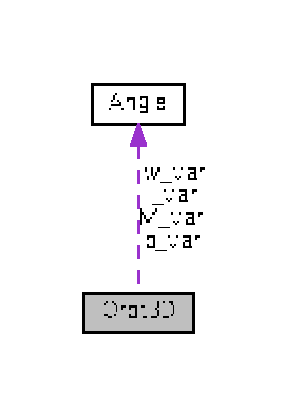
\includegraphics[width=139pt]{class_orbit3_d__coll__graph}
\end{center}
\end{figure}
\subsection*{Public Member Functions}
\begin{DoxyCompactItemize}
\item 
\hypertarget{class_orbit3_d_a35c5a9ed4b3cce05f74b35d0d430d388}{double \hyperlink{class_orbit3_d_a35c5a9ed4b3cce05f74b35d0d430d388}{e} () const }\label{class_orbit3_d_a35c5a9ed4b3cce05f74b35d0d430d388}

\begin{DoxyCompactList}\small\item\em Eccentricity. \end{DoxyCompactList}\item 
\hypertarget{class_orbit3_d_a35e1c0ac75c987273e6639fe800c941d}{void \hyperlink{class_orbit3_d_a35e1c0ac75c987273e6639fe800c941d}{e} (double newe)}\label{class_orbit3_d_a35e1c0ac75c987273e6639fe800c941d}

\begin{DoxyCompactList}\small\item\em Set Eccentricity. \end{DoxyCompactList}\item 
\hypertarget{class_orbit3_d_a4bbfb67fe34d59daf768c92ca782d80e}{double \hyperlink{class_orbit3_d_a4bbfb67fe34d59daf768c92ca782d80e}{eccentricity} () const }\label{class_orbit3_d_a4bbfb67fe34d59daf768c92ca782d80e}

\begin{DoxyCompactList}\small\item\em Alias of \hyperlink{class_orbit3_d_a35c5a9ed4b3cce05f74b35d0d430d388}{e()} \end{DoxyCompactList}\item 
\hypertarget{class_orbit3_d_ae566d2b93620b9427b123decf41ef171}{void \hyperlink{class_orbit3_d_ae566d2b93620b9427b123decf41ef171}{eccentricity} (double newe)}\label{class_orbit3_d_ae566d2b93620b9427b123decf41ef171}

\begin{DoxyCompactList}\small\item\em Alias of \hyperlink{class_orbit3_d_a35e1c0ac75c987273e6639fe800c941d}{e(double)} \end{DoxyCompactList}\item 
\hypertarget{class_orbit3_d_a0a08d23ce456665ac235bc6aac516868}{double \hyperlink{class_orbit3_d_a0a08d23ce456665ac235bc6aac516868}{a} () const }\label{class_orbit3_d_a0a08d23ce456665ac235bc6aac516868}

\begin{DoxyCompactList}\small\item\em Semi-\/major axis. \end{DoxyCompactList}\item 
\hypertarget{class_orbit3_d_ab6034b8f39402406da7cd4438af37021}{void \hyperlink{class_orbit3_d_ab6034b8f39402406da7cd4438af37021}{a} (double newa)}\label{class_orbit3_d_ab6034b8f39402406da7cd4438af37021}

\begin{DoxyCompactList}\small\item\em Set Semi-\/major axis. \end{DoxyCompactList}\item 
\hypertarget{class_orbit3_d_ab4ed5ce3b69df1c5832a7f0b3a0614be}{double \hyperlink{class_orbit3_d_ab4ed5ce3b69df1c5832a7f0b3a0614be}{semi\+Major\+Axis} () const }\label{class_orbit3_d_ab4ed5ce3b69df1c5832a7f0b3a0614be}

\begin{DoxyCompactList}\small\item\em Alias of \hyperlink{class_orbit3_d_a0a08d23ce456665ac235bc6aac516868}{a()} \end{DoxyCompactList}\item 
\hypertarget{class_orbit3_d_a0077a67a81517a1e5059c094cf0a0d87}{void \hyperlink{class_orbit3_d_a0077a67a81517a1e5059c094cf0a0d87}{semi\+Major\+Axis} (double newa)}\label{class_orbit3_d_a0077a67a81517a1e5059c094cf0a0d87}

\begin{DoxyCompactList}\small\item\em Alias of \hyperlink{class_orbit3_d_ab6034b8f39402406da7cd4438af37021}{a(double)} \end{DoxyCompactList}\item 
\hypertarget{class_orbit3_d_a041e5646cc9568695a931f39840e1c98}{\hyperlink{class_angle}{Angle} \hyperlink{class_orbit3_d_a041e5646cc9568695a931f39840e1c98}{i} () const }\label{class_orbit3_d_a041e5646cc9568695a931f39840e1c98}

\begin{DoxyCompactList}\small\item\em Inclination. \end{DoxyCompactList}\item 
\hypertarget{class_orbit3_d_a65a44009a60a004aad84cae0087c5f2e}{void \hyperlink{class_orbit3_d_a65a44009a60a004aad84cae0087c5f2e}{i} (\hyperlink{class_angle}{Angle} newi)}\label{class_orbit3_d_a65a44009a60a004aad84cae0087c5f2e}

\begin{DoxyCompactList}\small\item\em Set Inclination. \end{DoxyCompactList}\item 
\hypertarget{class_orbit3_d_afaf6886dcc7ffd5b8e73e6df8e9ecfc6}{\hyperlink{class_angle}{Angle} \hyperlink{class_orbit3_d_afaf6886dcc7ffd5b8e73e6df8e9ecfc6}{inclination} () const }\label{class_orbit3_d_afaf6886dcc7ffd5b8e73e6df8e9ecfc6}

\begin{DoxyCompactList}\small\item\em Alias of \hyperlink{class_orbit3_d_a041e5646cc9568695a931f39840e1c98}{i()} \end{DoxyCompactList}\item 
\hypertarget{class_orbit3_d_a580448e4199b0ac41f0024788b1c0dc2}{void \hyperlink{class_orbit3_d_a580448e4199b0ac41f0024788b1c0dc2}{inclination} (\hyperlink{class_angle}{Angle} newi)}\label{class_orbit3_d_a580448e4199b0ac41f0024788b1c0dc2}

\begin{DoxyCompactList}\small\item\em Alias of \hyperlink{class_orbit3_d_a65a44009a60a004aad84cae0087c5f2e}{i(\+Angle)} \end{DoxyCompactList}\item 
\hypertarget{class_orbit3_d_aec9343b132dc8d58e81ceaebf24951ec}{\hyperlink{class_angle}{Angle} \hyperlink{class_orbit3_d_aec9343b132dc8d58e81ceaebf24951ec}{o} () const }\label{class_orbit3_d_aec9343b132dc8d58e81ceaebf24951ec}

\begin{DoxyCompactList}\small\item\em Longitude of Ascending Node. \end{DoxyCompactList}\item 
\hypertarget{class_orbit3_d_a8f08e97baf48794a7891b1d53aa55b6e}{void \hyperlink{class_orbit3_d_a8f08e97baf48794a7891b1d53aa55b6e}{o} (\hyperlink{class_angle}{Angle} newo)}\label{class_orbit3_d_a8f08e97baf48794a7891b1d53aa55b6e}

\begin{DoxyCompactList}\small\item\em Set Longitude of Ascending Node. \end{DoxyCompactList}\item 
\hypertarget{class_orbit3_d_a772447fa58a0b5e36ae0d5dbd0bd62b5}{\hyperlink{class_angle}{Angle} \hyperlink{class_orbit3_d_a772447fa58a0b5e36ae0d5dbd0bd62b5}{w} () const }\label{class_orbit3_d_a772447fa58a0b5e36ae0d5dbd0bd62b5}

\begin{DoxyCompactList}\small\item\em Argument of periapsis. \end{DoxyCompactList}\item 
\hypertarget{class_orbit3_d_a6b89ee575430b0eaf7b7b53409c2808e}{void \hyperlink{class_orbit3_d_a6b89ee575430b0eaf7b7b53409c2808e}{w} (\hyperlink{class_angle}{Angle} neww)}\label{class_orbit3_d_a6b89ee575430b0eaf7b7b53409c2808e}

\begin{DoxyCompactList}\small\item\em Set Argument of periapsis. \end{DoxyCompactList}\item 
\hypertarget{class_orbit3_d_ae22e874a67bdb3e460266605c708f703}{\hyperlink{class_angle}{Angle} \hyperlink{class_orbit3_d_ae22e874a67bdb3e460266605c708f703}{argument\+Of\+Periapsis} () const }\label{class_orbit3_d_ae22e874a67bdb3e460266605c708f703}

\begin{DoxyCompactList}\small\item\em Alias of \hyperlink{class_orbit3_d_a772447fa58a0b5e36ae0d5dbd0bd62b5}{w()} \end{DoxyCompactList}\item 
\hypertarget{class_orbit3_d_a022c24e031b1f81261673b055ab4f320}{void \hyperlink{class_orbit3_d_a022c24e031b1f81261673b055ab4f320}{argument\+Of\+Periapsis} (\hyperlink{class_angle}{Angle} neww)}\label{class_orbit3_d_a022c24e031b1f81261673b055ab4f320}

\begin{DoxyCompactList}\small\item\em Alias of \hyperlink{class_orbit3_d_a6b89ee575430b0eaf7b7b53409c2808e}{w(\+Angle)} \end{DoxyCompactList}\item 
\hypertarget{class_orbit3_d_ac6eb0ccc3e3422d88210d0f4c8d56250}{\hyperlink{class_angle}{Angle} \hyperlink{class_orbit3_d_ac6eb0ccc3e3422d88210d0f4c8d56250}{M} () const }\label{class_orbit3_d_ac6eb0ccc3e3422d88210d0f4c8d56250}

\begin{DoxyCompactList}\small\item\em Mean Anomaly. \end{DoxyCompactList}\item 
\hypertarget{class_orbit3_d_abf5cf8df54ccd9fb475e9565ea2b422c}{void \hyperlink{class_orbit3_d_abf5cf8df54ccd9fb475e9565ea2b422c}{M} (\hyperlink{class_angle}{Angle} new\+M)}\label{class_orbit3_d_abf5cf8df54ccd9fb475e9565ea2b422c}

\begin{DoxyCompactList}\small\item\em Set Mean anomaly. \end{DoxyCompactList}\item 
\hypertarget{class_orbit3_d_ad4d38b96390a2a65579def92bfdb8895}{\hyperlink{class_angle}{Angle} \hyperlink{class_orbit3_d_ad4d38b96390a2a65579def92bfdb8895}{mean\+Anomaly} () const }\label{class_orbit3_d_ad4d38b96390a2a65579def92bfdb8895}

\begin{DoxyCompactList}\small\item\em Alias of \hyperlink{class_orbit3_d_ac6eb0ccc3e3422d88210d0f4c8d56250}{M()} \end{DoxyCompactList}\item 
\hypertarget{class_orbit3_d_a44b20386eba600bda7aa63486d31b9a9}{void \hyperlink{class_orbit3_d_a44b20386eba600bda7aa63486d31b9a9}{mean\+Anomaly} (\hyperlink{class_angle}{Angle} new\+M)}\label{class_orbit3_d_a44b20386eba600bda7aa63486d31b9a9}

\begin{DoxyCompactList}\small\item\em Alias of \hyperlink{class_orbit3_d_abf5cf8df54ccd9fb475e9565ea2b422c}{M(\+Angle)} \end{DoxyCompactList}\item 
double \hyperlink{class_orbit3_d_a2ba287a7401e69dd5181eb6bc2e44b24}{Peri\+And\+Apo\+Distance} () const 
\begin{DoxyCompactList}\small\item\em Returns r\+\_\+ap + r\+\_\+per. \end{DoxyCompactList}\item 
\hypertarget{class_orbit3_d_a305560357a9d598bc0d3d0d6841ec3c7}{double \hyperlink{class_orbit3_d_a305560357a9d598bc0d3d0d6841ec3c7}{r\+\_\+per} () const }\label{class_orbit3_d_a305560357a9d598bc0d3d0d6841ec3c7}

\begin{DoxyCompactList}\small\item\em Distance to Periapsis. \end{DoxyCompactList}\item 
\hypertarget{class_orbit3_d_a7021c6cde96f0b8aceccaa13dd6fbca5}{double \hyperlink{class_orbit3_d_a7021c6cde96f0b8aceccaa13dd6fbca5}{r\+\_\+ap} () const }\label{class_orbit3_d_a7021c6cde96f0b8aceccaa13dd6fbca5}

\begin{DoxyCompactList}\small\item\em Distance to Apoapsis. \end{DoxyCompactList}\item 
\hypertarget{class_orbit3_d_aecb936f5a84502c2d6254671b890ac92}{double \hyperlink{class_orbit3_d_aecb936f5a84502c2d6254671b890ac92}{Major\+Axis} () const }\label{class_orbit3_d_aecb936f5a84502c2d6254671b890ac92}

\begin{DoxyCompactList}\small\item\em Major axis. \end{DoxyCompactList}\item 
\hypertarget{class_orbit3_d_af395bba2ec4de8552ea8fafeed68189a}{double \hyperlink{class_orbit3_d_af395bba2ec4de8552ea8fafeed68189a}{b} () const }\label{class_orbit3_d_af395bba2ec4de8552ea8fafeed68189a}

\begin{DoxyCompactList}\small\item\em Semi Minor Axis. \end{DoxyCompactList}\item 
\hypertarget{class_orbit3_d_ad221ee0f571570c7b018a942ac49b513}{double \hyperlink{class_orbit3_d_ad221ee0f571570c7b018a942ac49b513}{semi\+Minor\+Axis} () const }\label{class_orbit3_d_ad221ee0f571570c7b018a942ac49b513}

\begin{DoxyCompactList}\small\item\em Alias of \hyperlink{class_orbit3_d_af395bba2ec4de8552ea8fafeed68189a}{b()} \end{DoxyCompactList}\item 
\hypertarget{class_orbit3_d_a08a9a86e2f5e074eb3bdda2efe9c56a0}{double \hyperlink{class_orbit3_d_a08a9a86e2f5e074eb3bdda2efe9c56a0}{Minor\+Axis} () const }\label{class_orbit3_d_a08a9a86e2f5e074eb3bdda2efe9c56a0}

\begin{DoxyCompactList}\small\item\em Minor Axis. \end{DoxyCompactList}\item 
\hypertarget{class_orbit3_d_a5f4c3402ffe5024fa383ccba9d9da88a}{double \hyperlink{class_orbit3_d_a5f4c3402ffe5024fa383ccba9d9da88a}{T} (double mew) const }\label{class_orbit3_d_a5f4c3402ffe5024fa383ccba9d9da88a}

\begin{DoxyCompactList}\small\item\em Orbital period. \end{DoxyCompactList}\item 
\hypertarget{class_orbit3_d_a2c19d1dd86d7feccfa8faa6e431aefd0}{double \hyperlink{class_orbit3_d_a2c19d1dd86d7feccfa8faa6e431aefd0}{orbital\+Period} (double mew) const }\label{class_orbit3_d_a2c19d1dd86d7feccfa8faa6e431aefd0}

\begin{DoxyCompactList}\small\item\em Alias of \hyperlink{class_orbit3_d_a5f4c3402ffe5024fa383ccba9d9da88a}{T()} \end{DoxyCompactList}\item 
double \hyperlink{class_orbit3_d_aca94003de3900c7e0353d44b6139bccd}{calculatea\+For\+Specific\+T} (double \hyperlink{class_orbit3_d_a5f4c3402ffe5024fa383ccba9d9da88a}{T}, double mew) const 
\begin{DoxyCompactList}\small\item\em Calculates semi-\/major axis required for selected orbital period. \end{DoxyCompactList}\item 
double \hyperlink{class_orbit3_d_ae3343982c02aa65cc8907aa825430ca7}{calculate\+Sync\+Orbit} (double srp, double mew) const 
\begin{DoxyCompactList}\small\item\em Calculates semi-\/major axis for synchronous orbit. \end{DoxyCompactList}\item 
\hyperlink{class_angle}{Angle} \hyperlink{class_orbit3_d_a0d34eaecc2589911c99e83fbc7534d4e}{u} () const 
\begin{DoxyCompactList}\small\item\em Argument of Latitude. \end{DoxyCompactList}\item 
\hypertarget{class_orbit3_d_adb582a3a80af66e68046b4079acb19da}{\hyperlink{class_angle}{Angle} \hyperlink{class_orbit3_d_adb582a3a80af66e68046b4079acb19da}{argument\+Of\+Latitude} () const }\label{class_orbit3_d_adb582a3a80af66e68046b4079acb19da}

\begin{DoxyCompactList}\small\item\em Alias of \hyperlink{class_orbit3_d_a0d34eaecc2589911c99e83fbc7534d4e}{u()} \end{DoxyCompactList}\item 
\hypertarget{class_orbit3_d_a45299ea39b36dd386012296ccbc228c1}{\hyperlink{class_angle}{Angle} \hyperlink{class_orbit3_d_a45299ea39b36dd386012296ccbc228c1}{l} () const }\label{class_orbit3_d_a45299ea39b36dd386012296ccbc228c1}

\begin{DoxyCompactList}\small\item\em True Longitude. \end{DoxyCompactList}\item 
\hypertarget{class_orbit3_d_aa6b53e359790913ebe55bc7af0a2c6e6}{\hyperlink{class_angle}{Angle} \hyperlink{class_orbit3_d_aa6b53e359790913ebe55bc7af0a2c6e6}{true\+Longitude} () const }\label{class_orbit3_d_aa6b53e359790913ebe55bc7af0a2c6e6}

\begin{DoxyCompactList}\small\item\em Alias of \hyperlink{class_orbit3_d_a45299ea39b36dd386012296ccbc228c1}{l()} \end{DoxyCompactList}\item 
\hyperlink{class_angle}{Angle} \hyperlink{class_orbit3_d_a9a6408ee7ee39feca254112bd0e3a398}{f} () const 
\begin{DoxyCompactList}\small\item\em True anomaly. \end{DoxyCompactList}\item 
\hypertarget{class_orbit3_d_aec33701fb9e7f5c4296482cd4f627598}{void \hyperlink{class_orbit3_d_aec33701fb9e7f5c4296482cd4f627598}{f} (\hyperlink{class_angle}{Angle} newf)}\label{class_orbit3_d_aec33701fb9e7f5c4296482cd4f627598}

\begin{DoxyCompactList}\small\item\em Set True anomaly. \end{DoxyCompactList}\item 
\hypertarget{class_orbit3_d_aa759bb74297b84e00a8f08af3558f212}{\hyperlink{class_angle}{Angle} \hyperlink{class_orbit3_d_aa759bb74297b84e00a8f08af3558f212}{true\+Anomaly} () const }\label{class_orbit3_d_aa759bb74297b84e00a8f08af3558f212}

\begin{DoxyCompactList}\small\item\em Alias of \hyperlink{class_orbit3_d_a9a6408ee7ee39feca254112bd0e3a398}{f()} \end{DoxyCompactList}\item 
\hypertarget{class_orbit3_d_adba90c3ed57af167019dcb12a40844e0}{void \hyperlink{class_orbit3_d_adba90c3ed57af167019dcb12a40844e0}{true\+Anomaly} (\hyperlink{class_angle}{Angle} newf)}\label{class_orbit3_d_adba90c3ed57af167019dcb12a40844e0}

\begin{DoxyCompactList}\small\item\em Alias of \hyperlink{class_orbit3_d_aec33701fb9e7f5c4296482cd4f627598}{f(\+Angle)} \end{DoxyCompactList}\item 
\hyperlink{class_angle}{Angle} \hyperlink{class_orbit3_d_a7ead8b6d4da1debda4f17a059b4749dd}{E} () const 
\begin{DoxyCompactList}\small\item\em Eccentric Anomaly. \end{DoxyCompactList}\item 
\hypertarget{class_orbit3_d_aa168d4ca33ef678204509adb0767826a}{\hyperlink{class_angle}{Angle} \hyperlink{class_orbit3_d_aa168d4ca33ef678204509adb0767826a}{eccentric\+Anomaly} () const }\label{class_orbit3_d_aa168d4ca33ef678204509adb0767826a}

\begin{DoxyCompactList}\small\item\em Alias of \hyperlink{class_orbit3_d_a7ead8b6d4da1debda4f17a059b4749dd}{E()} \end{DoxyCompactList}\item 
\hypertarget{class_orbit3_d_a6083fe36422073b1db449e6d13f49bd6}{double \hyperlink{class_orbit3_d_a6083fe36422073b1db449e6d13f49bd6}{ell} () const }\label{class_orbit3_d_a6083fe36422073b1db449e6d13f49bd6}

\begin{DoxyCompactList}\small\item\em Semi-\/\+Latus Rectum. \end{DoxyCompactList}\item 
\hypertarget{class_orbit3_d_ab4f68f04cdbe9316a38bb6feed107ca0}{double \hyperlink{class_orbit3_d_ab4f68f04cdbe9316a38bb6feed107ca0}{semi\+Latus\+Rectum} () const }\label{class_orbit3_d_ab4f68f04cdbe9316a38bb6feed107ca0}

\begin{DoxyCompactList}\small\item\em Alias of \hyperlink{class_orbit3_d_a6083fe36422073b1db449e6d13f49bd6}{ell()} \end{DoxyCompactList}\item 
\hypertarget{class_orbit3_d_accc97ffa7840ef5d83001d29f3d47140}{double \hyperlink{class_orbit3_d_accc97ffa7840ef5d83001d29f3d47140}{latus\+Rectum} () const }\label{class_orbit3_d_accc97ffa7840ef5d83001d29f3d47140}

\begin{DoxyCompactList}\small\item\em Latus Rectum. \end{DoxyCompactList}\item 
double \hyperlink{class_orbit3_d_ab2f6739b82102c7e525ce26ef22c631f}{p} () const 
\begin{DoxyCompactList}\small\item\em Focal Parameter. \end{DoxyCompactList}\item 
\hypertarget{class_orbit3_d_a2138a2a1bb8a08d73f01687952b82579}{double \hyperlink{class_orbit3_d_a2138a2a1bb8a08d73f01687952b82579}{focal\+Parameter} () const }\label{class_orbit3_d_a2138a2a1bb8a08d73f01687952b82579}

\begin{DoxyCompactList}\small\item\em Alias of \hyperlink{class_orbit3_d_ab2f6739b82102c7e525ce26ef22c631f}{p()} \end{DoxyCompactList}\item 
\hypertarget{class_orbit3_d_abb21ae1e48b886b134d3d06a7000d7ba}{Orbital\+Shape \hyperlink{class_orbit3_d_abb21ae1e48b886b134d3d06a7000d7ba}{shape} () const }\label{class_orbit3_d_abb21ae1e48b886b134d3d06a7000d7ba}

\begin{DoxyCompactList}\small\item\em Shape of Orbit. \end{DoxyCompactList}\item 
double \hyperlink{class_orbit3_d_a0660f58758e1461d7aaeff2684a950bd}{c} () const 
\begin{DoxyCompactList}\small\item\em Linear Eccentricity. \end{DoxyCompactList}\item 
\hypertarget{class_orbit3_d_a5eab9920c3c0a9adc716556e3a08f264}{double \hyperlink{class_orbit3_d_a5eab9920c3c0a9adc716556e3a08f264}{linear\+Eccentricity} () const }\label{class_orbit3_d_a5eab9920c3c0a9adc716556e3a08f264}

\begin{DoxyCompactList}\small\item\em Alias of \hyperlink{class_orbit3_d_a0660f58758e1461d7aaeff2684a950bd}{c()} \end{DoxyCompactList}\item 
\hypertarget{class_orbit3_d_aea1e7cfdd6e5709e3fe2dee8bf8aa33f}{double \hyperlink{class_orbit3_d_aea1e7cfdd6e5709e3fe2dee8bf8aa33f}{radius\+True\+Anomaly} () const }\label{class_orbit3_d_aea1e7cfdd6e5709e3fe2dee8bf8aa33f}

\begin{DoxyCompactList}\small\item\em Radius from True Anomaly. \end{DoxyCompactList}\item 
\hypertarget{class_orbit3_d_a7cb7c8c7777c4f208c1d586bab835be2}{double \hyperlink{class_orbit3_d_a7cb7c8c7777c4f208c1d586bab835be2}{radius\+Eccentric\+Anomaly} () const }\label{class_orbit3_d_a7cb7c8c7777c4f208c1d586bab835be2}

\begin{DoxyCompactList}\small\item\em Radius from Eccentric Anomaly. \end{DoxyCompactList}\item 
\hypertarget{class_orbit3_d_ada50a0694411e68f1a51ff62b3b63e91}{double \hyperlink{class_orbit3_d_ada50a0694411e68f1a51ff62b3b63e91}{epsilon} (double mew) const }\label{class_orbit3_d_ada50a0694411e68f1a51ff62b3b63e91}

\begin{DoxyCompactList}\small\item\em Specific Orbital Energy. \end{DoxyCompactList}\item 
\hypertarget{class_orbit3_d_acb4d6e994731789b845f077e1da67d36}{double \hyperlink{class_orbit3_d_acb4d6e994731789b845f077e1da67d36}{specific\+Orbital\+Energy} (double mew) const }\label{class_orbit3_d_acb4d6e994731789b845f077e1da67d36}

\begin{DoxyCompactList}\small\item\em Alias of \hyperlink{class_orbit3_d_ada50a0694411e68f1a51ff62b3b63e91}{epsilon()} \end{DoxyCompactList}\item 
\hypertarget{class_orbit3_d_aaa08afdb560b360dc721626e9a81161e}{double \hyperlink{class_orbit3_d_aaa08afdb560b360dc721626e9a81161e}{v} (double mew) const }\label{class_orbit3_d_aaa08afdb560b360dc721626e9a81161e}

\begin{DoxyCompactList}\small\item\em Mean Orbital Speed. \end{DoxyCompactList}\item 
\hypertarget{class_orbit3_d_aa8e2de96cf1ec1b7695ea884df03a9c7}{double \hyperlink{class_orbit3_d_aa8e2de96cf1ec1b7695ea884df03a9c7}{mean\+Orbital\+Speed} (double mew) const }\label{class_orbit3_d_aa8e2de96cf1ec1b7695ea884df03a9c7}

\begin{DoxyCompactList}\small\item\em Alias of v(double) \end{DoxyCompactList}\item 
\hypertarget{class_orbit3_d_a45a7c59fe4276f2a5bc5343caa7ca5ee}{\hyperlink{class_vector3_d}{Vector3\+D} \hyperlink{class_orbit3_d_a45a7c59fe4276f2a5bc5343caa7ca5ee}{h\+Bar} () const }\label{class_orbit3_d_a45a7c59fe4276f2a5bc5343caa7ca5ee}

\begin{DoxyCompactList}\small\item\em Specific Relative Angular Momentum. \end{DoxyCompactList}\item 
\hypertarget{class_orbit3_d_a24e8d26cbf5723538d62940caae960a0}{\hyperlink{class_vector3_d}{Vector3\+D} \hyperlink{class_orbit3_d_a24e8d26cbf5723538d62940caae960a0}{specific\+Relative\+Angular\+Momentum} () const }\label{class_orbit3_d_a24e8d26cbf5723538d62940caae960a0}

\begin{DoxyCompactList}\small\item\em Alias of \hyperlink{class_orbit3_d_a45a7c59fe4276f2a5bc5343caa7ca5ee}{h\+Bar()} \end{DoxyCompactList}\item 
\hypertarget{class_orbit3_d_ab892cbfb91cf58d6145fcc4457a4ed17}{\hyperlink{class_vector3_d}{Vector3\+D} \hyperlink{class_orbit3_d_ab892cbfb91cf58d6145fcc4457a4ed17}{osvr} () const }\label{class_orbit3_d_ab892cbfb91cf58d6145fcc4457a4ed17}

\begin{DoxyCompactList}\small\item\em Orbital state vector position. \end{DoxyCompactList}\item 
\hypertarget{class_orbit3_d_a73b48753675733e273a36faf2291eefa}{\hyperlink{class_vector3_d}{Vector3\+D} \hyperlink{class_orbit3_d_a73b48753675733e273a36faf2291eefa}{osvv} () const }\label{class_orbit3_d_a73b48753675733e273a36faf2291eefa}

\begin{DoxyCompactList}\small\item\em Orbital state vector velocity. \end{DoxyCompactList}\item 
\hypertarget{class_orbit3_d_a0c48a720152f61990498eb8ceb79a8a7}{\hyperlink{class_vector3_d}{Vector3\+D} \hyperlink{class_orbit3_d_a0c48a720152f61990498eb8ceb79a8a7}{line\+Of\+Nodes} () const }\label{class_orbit3_d_a0c48a720152f61990498eb8ceb79a8a7}

\begin{DoxyCompactList}\small\item\em Line of nodes vector. \end{DoxyCompactList}\item 
\hypertarget{class_orbit3_d_a9319326e1a214e644fc383c898713ef6}{double \hyperlink{class_orbit3_d_a9319326e1a214e644fc383c898713ef6}{n} (double mew) const }\label{class_orbit3_d_a9319326e1a214e644fc383c898713ef6}

\begin{DoxyCompactList}\small\item\em Mean Motion. \end{DoxyCompactList}\item 
\hypertarget{class_orbit3_d_a8fd3eb6ad07a8111f4746dd3be6d86a2}{double \hyperlink{class_orbit3_d_a8fd3eb6ad07a8111f4746dd3be6d86a2}{mean\+Motion} (double mew) const }\label{class_orbit3_d_a8fd3eb6ad07a8111f4746dd3be6d86a2}

\begin{DoxyCompactList}\small\item\em Alias of n(double) \end{DoxyCompactList}\item 
\hypertarget{class_orbit3_d_a5c045adcbffa82f43988d25d0962bf5f}{double \hyperlink{class_orbit3_d_a5c045adcbffa82f43988d25d0962bf5f}{mean\+Longitude} () const }\label{class_orbit3_d_a5c045adcbffa82f43988d25d0962bf5f}

\begin{DoxyCompactList}\small\item\em Mean longitude. \end{DoxyCompactList}\item 
\hypertarget{class_orbit3_d_af04e2f2b465bbf37ab97d045c88effda}{double \hyperlink{class_orbit3_d_af04e2f2b465bbf37ab97d045c88effda}{longitude\+Of\+Periapsis} () const }\label{class_orbit3_d_af04e2f2b465bbf37ab97d045c88effda}

\begin{DoxyCompactList}\small\item\em Longitude of Periapsis. \end{DoxyCompactList}\item 
\hypertarget{class_orbit3_d_a931c59f5a553cf2ddb0418ee30c3246b}{\hyperlink{class_vector3_d}{Vector3\+D} \hyperlink{class_orbit3_d_a931c59f5a553cf2ddb0418ee30c3246b}{h} () const }\label{class_orbit3_d_a931c59f5a553cf2ddb0418ee30c3246b}

\begin{DoxyCompactList}\small\item\em Angular Momentum. \end{DoxyCompactList}\item 
\hypertarget{class_orbit3_d_ab24851fadd30d88880e63c77fb8c8a34}{\hyperlink{class_vector3_d}{Vector3\+D} \hyperlink{class_orbit3_d_ab24851fadd30d88880e63c77fb8c8a34}{angular\+Momentum} () const }\label{class_orbit3_d_ab24851fadd30d88880e63c77fb8c8a34}

\begin{DoxyCompactList}\small\item\em Alias of \hyperlink{class_orbit3_d_a931c59f5a553cf2ddb0418ee30c3246b}{h()} \end{DoxyCompactList}\end{DoxyCompactItemize}
\subsection*{Protected Attributes}
\begin{DoxyCompactItemize}
\item 
\hypertarget{class_orbit3_d_a573611da3b62dd90339c6c09dbafe881}{double \hyperlink{class_orbit3_d_a573611da3b62dd90339c6c09dbafe881}{e\+\_\+var}}\label{class_orbit3_d_a573611da3b62dd90339c6c09dbafe881}

\begin{DoxyCompactList}\small\item\em Eccentricity. \end{DoxyCompactList}\item 
\hypertarget{class_orbit3_d_aae4380c7fec444703aae70199537e6ad}{double \hyperlink{class_orbit3_d_aae4380c7fec444703aae70199537e6ad}{a\+\_\+var}}\label{class_orbit3_d_aae4380c7fec444703aae70199537e6ad}

\begin{DoxyCompactList}\small\item\em Semi-\/major axis. \end{DoxyCompactList}\item 
\hypertarget{class_orbit3_d_a31eb6dd2995ec28130e04f01e8fa7085}{\hyperlink{class_angle}{Angle} \hyperlink{class_orbit3_d_a31eb6dd2995ec28130e04f01e8fa7085}{i\+\_\+var}}\label{class_orbit3_d_a31eb6dd2995ec28130e04f01e8fa7085}

\begin{DoxyCompactList}\small\item\em Inclination. \end{DoxyCompactList}\item 
\hypertarget{class_orbit3_d_a28391400bb3ad7f2ec5eb85edfa2eeb0}{\hyperlink{class_angle}{Angle} \hyperlink{class_orbit3_d_a28391400bb3ad7f2ec5eb85edfa2eeb0}{o\+\_\+var}}\label{class_orbit3_d_a28391400bb3ad7f2ec5eb85edfa2eeb0}

\begin{DoxyCompactList}\small\item\em Longitude of Ascending Node. \end{DoxyCompactList}\item 
\hypertarget{class_orbit3_d_a15c064c8739446d98728744405b0da63}{\hyperlink{class_angle}{Angle} \hyperlink{class_orbit3_d_a15c064c8739446d98728744405b0da63}{w\+\_\+var}}\label{class_orbit3_d_a15c064c8739446d98728744405b0da63}

\begin{DoxyCompactList}\small\item\em Argument of periapsis. \end{DoxyCompactList}\item 
\hypertarget{class_orbit3_d_a37deb92c6212b9452a4ade9d8faeb133}{\hyperlink{class_angle}{Angle} \hyperlink{class_orbit3_d_a37deb92c6212b9452a4ade9d8faeb133}{M\+\_\+var}}\label{class_orbit3_d_a37deb92c6212b9452a4ade9d8faeb133}

\begin{DoxyCompactList}\small\item\em Mean anomaly. \end{DoxyCompactList}\end{DoxyCompactItemize}


\subsection{Detailed Description}
Represents an orbit around an unspecified central body. 

This class defines an orbit around a central body using Keplerian elements. The elements used to define the orbit are the eccentricity, semi-\/major axis, inclination, longitude of ascending node, argument of periapsis, and mean anomaly.

All other return values are calculated in terms of these elements. The Standard Gravitational Parameter (mew) is required to calculate any elements that are based on the mass of the planet. 

\subsection{Member Function Documentation}
\hypertarget{class_orbit3_d_a0660f58758e1461d7aaeff2684a950bd}{\index{Orbit3\+D@{Orbit3\+D}!c@{c}}
\index{c@{c}!Orbit3\+D@{Orbit3\+D}}
\subsubsection[{c}]{\setlength{\rightskip}{0pt plus 5cm}double Orbit3\+D\+::c (
\begin{DoxyParamCaption}
{}
\end{DoxyParamCaption}
) const}}\label{class_orbit3_d_a0660f58758e1461d7aaeff2684a950bd}


Linear Eccentricity. 

This is undefined for parabolic orbits and this function will throw an exception \hypertarget{class_orbit3_d_aca94003de3900c7e0353d44b6139bccd}{\index{Orbit3\+D@{Orbit3\+D}!calculatea\+For\+Specific\+T@{calculatea\+For\+Specific\+T}}
\index{calculatea\+For\+Specific\+T@{calculatea\+For\+Specific\+T}!Orbit3\+D@{Orbit3\+D}}
\subsubsection[{calculatea\+For\+Specific\+T}]{\setlength{\rightskip}{0pt plus 5cm}double Orbit3\+D\+::calculatea\+For\+Specific\+T (
\begin{DoxyParamCaption}
\item[{double}]{T, }
\item[{double}]{mew}
\end{DoxyParamCaption}
) const}}\label{class_orbit3_d_aca94003de3900c7e0353d44b6139bccd}


Calculates semi-\/major axis required for selected orbital period. 


\begin{DoxyParams}{Parameters}
{\em T} & The amount of time in seconds \\
\hline
\end{DoxyParams}
\hypertarget{class_orbit3_d_ae3343982c02aa65cc8907aa825430ca7}{\index{Orbit3\+D@{Orbit3\+D}!calculate\+Sync\+Orbit@{calculate\+Sync\+Orbit}}
\index{calculate\+Sync\+Orbit@{calculate\+Sync\+Orbit}!Orbit3\+D@{Orbit3\+D}}
\subsubsection[{calculate\+Sync\+Orbit}]{\setlength{\rightskip}{0pt plus 5cm}double Orbit3\+D\+::calculate\+Sync\+Orbit (
\begin{DoxyParamCaption}
\item[{double}]{srp, }
\item[{double}]{mew}
\end{DoxyParamCaption}
) const\hspace{0.3cm}{\ttfamily [inline]}}}\label{class_orbit3_d_ae3343982c02aa65cc8907aa825430ca7}


Calculates semi-\/major axis for synchronous orbit. 


\begin{DoxyParams}{Parameters}
{\em srp} & The time it takes for one rotation in seconds \\
\hline
\end{DoxyParams}
\hypertarget{class_orbit3_d_a7ead8b6d4da1debda4f17a059b4749dd}{\index{Orbit3\+D@{Orbit3\+D}!E@{E}}
\index{E@{E}!Orbit3\+D@{Orbit3\+D}}
\subsubsection[{E}]{\setlength{\rightskip}{0pt plus 5cm}{\bf Angle} Orbit3\+D\+::\+E (
\begin{DoxyParamCaption}
{}
\end{DoxyParamCaption}
) const}}\label{class_orbit3_d_a7ead8b6d4da1debda4f17a059b4749dd}


Eccentric Anomaly. 

Calculated using Newton's method \hypertarget{class_orbit3_d_a9a6408ee7ee39feca254112bd0e3a398}{\index{Orbit3\+D@{Orbit3\+D}!f@{f}}
\index{f@{f}!Orbit3\+D@{Orbit3\+D}}
\subsubsection[{f}]{\setlength{\rightskip}{0pt plus 5cm}{\bf Angle} Orbit3\+D\+::f (
\begin{DoxyParamCaption}
{}
\end{DoxyParamCaption}
) const}}\label{class_orbit3_d_a9a6408ee7ee39feca254112bd0e3a398}


True anomaly. 

Undefined in circular orbits, use \hyperlink{class_orbit3_d_adb582a3a80af66e68046b4079acb19da}{argument\+Of\+Latitude()} \hypertarget{class_orbit3_d_ab2f6739b82102c7e525ce26ef22c631f}{\index{Orbit3\+D@{Orbit3\+D}!p@{p}}
\index{p@{p}!Orbit3\+D@{Orbit3\+D}}
\subsubsection[{p}]{\setlength{\rightskip}{0pt plus 5cm}double Orbit3\+D\+::p (
\begin{DoxyParamCaption}
{}
\end{DoxyParamCaption}
) const}}\label{class_orbit3_d_ab2f6739b82102c7e525ce26ef22c631f}


Focal Parameter. 

Focal parameter is infinite for circular orbits and this function will throw an exception. \hypertarget{class_orbit3_d_a2ba287a7401e69dd5181eb6bc2e44b24}{\index{Orbit3\+D@{Orbit3\+D}!Peri\+And\+Apo\+Distance@{Peri\+And\+Apo\+Distance}}
\index{Peri\+And\+Apo\+Distance@{Peri\+And\+Apo\+Distance}!Orbit3\+D@{Orbit3\+D}}
\subsubsection[{Peri\+And\+Apo\+Distance}]{\setlength{\rightskip}{0pt plus 5cm}double Orbit3\+D\+::\+Peri\+And\+Apo\+Distance (
\begin{DoxyParamCaption}
{}
\end{DoxyParamCaption}
) const}}\label{class_orbit3_d_a2ba287a7401e69dd5181eb6bc2e44b24}


Returns r\+\_\+ap + r\+\_\+per. 

Divides the semi-\/major axis by 2 giving the sum of the distance between the apoapsis and periapsis. \hypertarget{class_orbit3_d_a0d34eaecc2589911c99e83fbc7534d4e}{\index{Orbit3\+D@{Orbit3\+D}!u@{u}}
\index{u@{u}!Orbit3\+D@{Orbit3\+D}}
\subsubsection[{u}]{\setlength{\rightskip}{0pt plus 5cm}{\bf Angle} Orbit3\+D\+::u (
\begin{DoxyParamCaption}
{}
\end{DoxyParamCaption}
) const}}\label{class_orbit3_d_a0d34eaecc2589911c99e83fbc7534d4e}


Argument of Latitude. 

Undefined in circular orbits with zero inclination, use \hyperlink{class_orbit3_d_aa6b53e359790913ebe55bc7af0a2c6e6}{true\+Longitude()} 

The documentation for this class was generated from the following files\+:\begin{DoxyCompactItemize}
\item 
include/Orbit3\+D.\+h\item 
src/Orbit3\+D.\+cpp\end{DoxyCompactItemize}

\hypertarget{class_point3_d}{\section{Point3\+D Class Reference}
\label{class_point3_d}\index{Point3\+D@{Point3\+D}}
}


A point in 3-\/dimensional space.  




{\ttfamily \#include $<$Point3\+D.\+h$>$}



Inheritance diagram for Point3\+D\+:\nopagebreak
\begin{figure}[H]
\begin{center}
\leavevmode
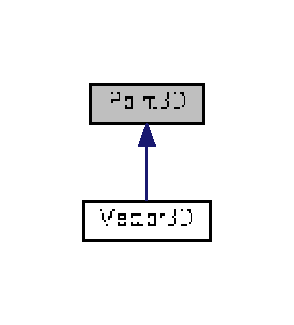
\includegraphics[width=141pt]{class_point3_d__inherit__graph}
\end{center}
\end{figure}
\subsection*{Public Member Functions}
\begin{DoxyCompactItemize}
\item 
\hypertarget{class_point3_d_ada3b28b2c868649ad4d68e9001b3d991}{double \hyperlink{class_point3_d_ada3b28b2c868649ad4d68e9001b3d991}{x} () const }\label{class_point3_d_ada3b28b2c868649ad4d68e9001b3d991}

\begin{DoxyCompactList}\small\item\em Get coord x. \end{DoxyCompactList}\item 
\hypertarget{class_point3_d_a8289fc2d572ccba7f605b9fbe7225b46}{void \hyperlink{class_point3_d_a8289fc2d572ccba7f605b9fbe7225b46}{x} (double newx)}\label{class_point3_d_a8289fc2d572ccba7f605b9fbe7225b46}

\begin{DoxyCompactList}\small\item\em Set coord x. \end{DoxyCompactList}\item 
\hypertarget{class_point3_d_afcabb8cbb3e5ef969f7e6117d4b85496}{double \hyperlink{class_point3_d_afcabb8cbb3e5ef969f7e6117d4b85496}{y} () const }\label{class_point3_d_afcabb8cbb3e5ef969f7e6117d4b85496}

\begin{DoxyCompactList}\small\item\em Get coord y. \end{DoxyCompactList}\item 
\hypertarget{class_point3_d_a3cbeb175d16bd3067569115f7e026fd3}{void \hyperlink{class_point3_d_a3cbeb175d16bd3067569115f7e026fd3}{y} (double newy)}\label{class_point3_d_a3cbeb175d16bd3067569115f7e026fd3}

\begin{DoxyCompactList}\small\item\em Set coord y. \end{DoxyCompactList}\item 
\hypertarget{class_point3_d_ab2c30268a9b50d54ed1ae8285bedd931}{double \hyperlink{class_point3_d_ab2c30268a9b50d54ed1ae8285bedd931}{z} () const }\label{class_point3_d_ab2c30268a9b50d54ed1ae8285bedd931}

\begin{DoxyCompactList}\small\item\em Get coord z. \end{DoxyCompactList}\item 
\hypertarget{class_point3_d_a98dac6c2cac54f7d34ae6f23e6bcaf93}{void \hyperlink{class_point3_d_a98dac6c2cac54f7d34ae6f23e6bcaf93}{z} (double newz)}\label{class_point3_d_a98dac6c2cac54f7d34ae6f23e6bcaf93}

\begin{DoxyCompactList}\small\item\em Set coord z. \end{DoxyCompactList}\end{DoxyCompactItemize}


\subsection{Detailed Description}
A point in 3-\/dimensional space. 

The documentation for this class was generated from the following files\+:\begin{DoxyCompactItemize}
\item 
include/Point3\+D.\+h\item 
src/Point3\+D.\+cpp\end{DoxyCompactItemize}

\hypertarget{class_vector3_d}{\section{Vector3\+D Class Reference}
\label{class_vector3_d}\index{Vector3\+D@{Vector3\+D}}
}


A vector in 3-\/dimensional space.  




{\ttfamily \#include $<$Vector3\+D.\+h$>$}



Inheritance diagram for Vector3\+D\+:\nopagebreak
\begin{figure}[H]
\begin{center}
\leavevmode
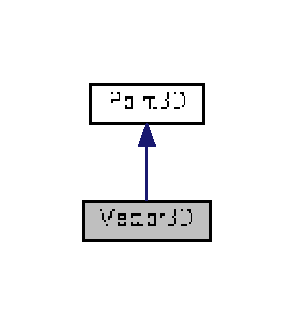
\includegraphics[width=141pt]{class_vector3_d__inherit__graph}
\end{center}
\end{figure}


Collaboration diagram for Vector3\+D\+:\nopagebreak
\begin{figure}[H]
\begin{center}
\leavevmode
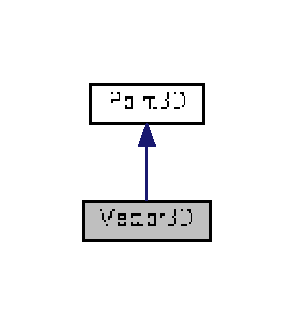
\includegraphics[width=141pt]{class_vector3_d__coll__graph}
\end{center}
\end{figure}
\subsection*{Public Member Functions}
\begin{DoxyCompactItemize}
\item 
\hypertarget{class_vector3_d_a2d02adba0f730e11fc64f6c3088e961c}{\hyperlink{class_vector3_d_a2d02adba0f730e11fc64f6c3088e961c}{Vector3\+D} (double newx, double newy, double newz)}\label{class_vector3_d_a2d02adba0f730e11fc64f6c3088e961c}

\begin{DoxyCompactList}\small\item\em Constructor with coordinates. \end{DoxyCompactList}\item 
\hypertarget{class_vector3_d_a0b11a8d75da427b27443d8a94d0d296c}{\hyperlink{class_vector3_d_a0b11a8d75da427b27443d8a94d0d296c}{Vector3\+D} ()}\label{class_vector3_d_a0b11a8d75da427b27443d8a94d0d296c}

\begin{DoxyCompactList}\small\item\em Default constructor, makes zero vector. \end{DoxyCompactList}\item 
\hypertarget{class_vector3_d_ab0356b9f5bd4be1156bd533cc82ee1af}{\hyperlink{class_vector3_d_ab0356b9f5bd4be1156bd533cc82ee1af}{Vector3\+D} (\hyperlink{class_point3_d}{Point3\+D} p1, \hyperlink{class_point3_d}{Point3\+D} p2)}\label{class_vector3_d_ab0356b9f5bd4be1156bd533cc82ee1af}

\begin{DoxyCompactList}\small\item\em Create a vector representing 2 sets of coordinates. \end{DoxyCompactList}\item 
\hypertarget{class_vector3_d_a84165b911b5ae2c281a95d1bd60ecc4a}{\hyperlink{class_angle}{Angle} \hyperlink{class_vector3_d_a84165b911b5ae2c281a95d1bd60ecc4a}{alpha} () const }\label{class_vector3_d_a84165b911b5ae2c281a95d1bd60ecc4a}

\begin{DoxyCompactList}\small\item\em \hyperlink{class_angle}{Angle} from x axis to vector. \end{DoxyCompactList}\item 
\hypertarget{class_vector3_d_ae6572e98df6b70b759c85c87031bd9ed}{void \hyperlink{class_vector3_d_ae6572e98df6b70b759c85c87031bd9ed}{alpha} (\hyperlink{class_angle}{Angle} newa)}\label{class_vector3_d_ae6572e98df6b70b759c85c87031bd9ed}

\begin{DoxyCompactList}\small\item\em Modify alpha angle. \end{DoxyCompactList}\item 
\hypertarget{class_vector3_d_a49fc7ce9e4ccfacd29c5d93c8f6e408b}{\hyperlink{class_angle}{Angle} \hyperlink{class_vector3_d_a49fc7ce9e4ccfacd29c5d93c8f6e408b}{beta} () const }\label{class_vector3_d_a49fc7ce9e4ccfacd29c5d93c8f6e408b}

\begin{DoxyCompactList}\small\item\em \hyperlink{class_angle}{Angle} from y axis to vector. \end{DoxyCompactList}\item 
\hypertarget{class_vector3_d_a560bce5059d32a17e57136bb0f050147}{void \hyperlink{class_vector3_d_a560bce5059d32a17e57136bb0f050147}{beta} (\hyperlink{class_angle}{Angle} newa)}\label{class_vector3_d_a560bce5059d32a17e57136bb0f050147}

\begin{DoxyCompactList}\small\item\em Modify beta angle. \end{DoxyCompactList}\item 
\hypertarget{class_vector3_d_a70ef6a5eabcd9305fe2c779600f817d7}{\hyperlink{class_angle}{Angle} \hyperlink{class_vector3_d_a70ef6a5eabcd9305fe2c779600f817d7}{gamma} () const }\label{class_vector3_d_a70ef6a5eabcd9305fe2c779600f817d7}

\begin{DoxyCompactList}\small\item\em \hyperlink{class_angle}{Angle} from z axis to vector. \end{DoxyCompactList}\item 
\hypertarget{class_vector3_d_a6a213d186a1251fcedd3ecbe506ca6d0}{void \hyperlink{class_vector3_d_a6a213d186a1251fcedd3ecbe506ca6d0}{gamma} (\hyperlink{class_angle}{Angle} newa)}\label{class_vector3_d_a6a213d186a1251fcedd3ecbe506ca6d0}

\begin{DoxyCompactList}\small\item\em Modify gamma angle. \end{DoxyCompactList}\item 
\hypertarget{class_vector3_d_a9d168a5ff47377f6152f34d67324490d}{\hyperlink{class_angle}{Angle} \hyperlink{class_vector3_d_a9d168a5ff47377f6152f34d67324490d}{theta} () const }\label{class_vector3_d_a9d168a5ff47377f6152f34d67324490d}

\begin{DoxyCompactList}\small\item\em \hyperlink{class_angle}{Angle} from z axis to vector. \end{DoxyCompactList}\item 
\hypertarget{class_vector3_d_a84fef530c6610b732957788da80e42f3}{\hyperlink{class_angle}{Angle} \hyperlink{class_vector3_d_a84fef530c6610b732957788da80e42f3}{phi} () const }\label{class_vector3_d_a84fef530c6610b732957788da80e42f3}

\begin{DoxyCompactList}\small\item\em \hyperlink{class_angle}{Angle} from x axis to 2\+D vector. \end{DoxyCompactList}\item 
\hypertarget{class_vector3_d_ac5b3b5fdce5c8de7a405e731ea2825ba}{double \hyperlink{class_vector3_d_ac5b3b5fdce5c8de7a405e731ea2825ba}{magnitude} () const }\label{class_vector3_d_ac5b3b5fdce5c8de7a405e731ea2825ba}

\begin{DoxyCompactList}\small\item\em Returns magnitude of vector. \end{DoxyCompactList}\item 
\hypertarget{class_vector3_d_a93ac7c02548274417286170cc26b18f4}{bool \hyperlink{class_vector3_d_a93ac7c02548274417286170cc26b18f4}{is\+Zero} () const }\label{class_vector3_d_a93ac7c02548274417286170cc26b18f4}

\begin{DoxyCompactList}\small\item\em Checks if vector has no magnitude or direction. \end{DoxyCompactList}\item 
\hypertarget{class_vector3_d_a1cd7d48d3e97fc2d6764968865f6a7ec}{bool \hyperlink{class_vector3_d_a1cd7d48d3e97fc2d6764968865f6a7ec}{is\+Unit} () const }\label{class_vector3_d_a1cd7d48d3e97fc2d6764968865f6a7ec}

\begin{DoxyCompactList}\small\item\em Check if vector magnitude is 1. \end{DoxyCompactList}\item 
\hypertarget{class_vector3_d_a35b4835bfa487fe3d92f86ca591188fe}{bool \hyperlink{class_vector3_d_a35b4835bfa487fe3d92f86ca591188fe}{operator==} (const \hyperlink{class_vector3_d}{Vector3\+D} b) const }\label{class_vector3_d_a35b4835bfa487fe3d92f86ca591188fe}

\begin{DoxyCompactList}\small\item\em Allows vectors to be compared. \end{DoxyCompactList}\item 
\hypertarget{class_vector3_d_ac7c47cbae1aa443c138afc93daae815a}{bool \hyperlink{class_vector3_d_ac7c47cbae1aa443c138afc93daae815a}{is\+Opposite} (const \hyperlink{class_vector3_d}{Vector3\+D} b) const }\label{class_vector3_d_ac7c47cbae1aa443c138afc93daae815a}

\begin{DoxyCompactList}\small\item\em Checks if vector is opposite. \end{DoxyCompactList}\item 
\hypertarget{class_vector3_d_aa7318735a351a17f1c4108790e950303}{bool \hyperlink{class_vector3_d_aa7318735a351a17f1c4108790e950303}{is\+Parallel} (const \hyperlink{class_vector3_d}{Vector3\+D} b) const }\label{class_vector3_d_aa7318735a351a17f1c4108790e950303}

\begin{DoxyCompactList}\small\item\em Checks if vector is parallel. \end{DoxyCompactList}\item 
\hypertarget{class_vector3_d_a745d1d89cf74295a561e33db335a4f38}{bool \hyperlink{class_vector3_d_a745d1d89cf74295a561e33db335a4f38}{is\+Antiparallel} (const \hyperlink{class_vector3_d}{Vector3\+D} b) const }\label{class_vector3_d_a745d1d89cf74295a561e33db335a4f38}

\begin{DoxyCompactList}\small\item\em Checks if vector is anitparallel. \end{DoxyCompactList}\item 
\hypertarget{class_vector3_d_a7d46b011b385bfaf111e9fbba99aa89b}{\hyperlink{class_vector3_d}{Vector3\+D} \hyperlink{class_vector3_d_a7d46b011b385bfaf111e9fbba99aa89b}{operator+} (const \hyperlink{class_vector3_d}{Vector3\+D} \&b) const }\label{class_vector3_d_a7d46b011b385bfaf111e9fbba99aa89b}

\begin{DoxyCompactList}\small\item\em Allows vectors to be added. \end{DoxyCompactList}\item 
\hypertarget{class_vector3_d_a5a871906d907637c0f8f22a01430e118}{\hyperlink{class_vector3_d}{Vector3\+D} \hyperlink{class_vector3_d_a5a871906d907637c0f8f22a01430e118}{operator-\/} (const \hyperlink{class_vector3_d}{Vector3\+D} \&b) const }\label{class_vector3_d_a5a871906d907637c0f8f22a01430e118}

\begin{DoxyCompactList}\small\item\em Allows vectors to be subtracted. \end{DoxyCompactList}\item 
\hypertarget{class_vector3_d_acb77478f27bcb44bab94a8b8610327ad}{\hyperlink{class_vector3_d}{Vector3\+D} \hyperlink{class_vector3_d_acb77478f27bcb44bab94a8b8610327ad}{operator$\ast$} (const double \&b) const }\label{class_vector3_d_acb77478f27bcb44bab94a8b8610327ad}

\begin{DoxyCompactList}\small\item\em Allows multiply vector by scalar. \end{DoxyCompactList}\item 
\hypertarget{class_vector3_d_afd918fd5c482a98b44b9451a0936dc0c}{\hyperlink{class_vector3_d}{Vector3\+D} \hyperlink{class_vector3_d_afd918fd5c482a98b44b9451a0936dc0c}{operator/} (const double \&b) const }\label{class_vector3_d_afd918fd5c482a98b44b9451a0936dc0c}

\begin{DoxyCompactList}\small\item\em Allows division vector by scalar. \end{DoxyCompactList}\item 
\hypertarget{class_vector3_d_a4cd2ffbcf4d714a07586dd4c545c3434}{double \hyperlink{class_vector3_d_a4cd2ffbcf4d714a07586dd4c545c3434}{dot\+Product} (const \hyperlink{class_vector3_d}{Vector3\+D} b) const }\label{class_vector3_d_a4cd2ffbcf4d714a07586dd4c545c3434}

\begin{DoxyCompactList}\small\item\em Generate dot product of 2 vectors. \end{DoxyCompactList}\item 
\hypertarget{class_vector3_d_a564d7170bafa8ac8e325603742eddc94}{\hyperlink{class_vector3_d}{Vector3\+D} \hyperlink{class_vector3_d_a564d7170bafa8ac8e325603742eddc94}{cross\+Product} (const \hyperlink{class_vector3_d}{Vector3\+D} b) const }\label{class_vector3_d_a564d7170bafa8ac8e325603742eddc94}

\begin{DoxyCompactList}\small\item\em Generate cross product of 2 vectors. \end{DoxyCompactList}\item 
\hypertarget{class_vector3_d_ac56e4b6a4eb4e39f344187e2ef085435}{\hyperlink{class_angle}{Angle} \hyperlink{class_vector3_d_ac56e4b6a4eb4e39f344187e2ef085435}{find\+Angle} (const \hyperlink{class_vector3_d}{Vector3\+D} b) const }\label{class_vector3_d_ac56e4b6a4eb4e39f344187e2ef085435}

\begin{DoxyCompactList}\small\item\em Calculate angle between 2 vectors. \end{DoxyCompactList}\end{DoxyCompactItemize}


\subsection{Detailed Description}
A vector in 3-\/dimensional space. 

The documentation for this class was generated from the following files\+:\begin{DoxyCompactItemize}
\item 
include/Vector3\+D.\+h\item 
src/Vector3\+D.\+cpp\end{DoxyCompactItemize}

%--- End generated contents ---

% Index
\newpage
\phantomsection
\addcontentsline{toc}{chapter}{Index}
\printindex

\end{document}
